% Define the module top matter
% This gets used to create the chapter title page
% NOTES:
%  * When multiple people have authored or contributed to the module, simply use a LaTeX line break
%    (a double-backslash: \\) at the end of each person.
%  * If you don't want this information shown on the module chapter page, simply remove the lines
%    within the \setModuleAuthors{} and \setModuleContributions{} environments
\setModuleTitle{Introduction to Nextflow}
\setModuleAuthors{%
  Rados{\l}aw Suchecki \mailto{rad.suchecki@csiro.au}
}
\setModuleContributions{
Nathan S. Watson-Haigh \mailto{nathan.watson-haigh@adelaide.edu.au}
}

% BEGIN: Module Title Page
% This simply uses the above information and creates a module chapter page
% NOTES:
%  * The chapter page will always appear on odd numbered page
\chapter{\moduleTitle}
\newpage
% END: Module Title Page


% BEGIN: KLOs
% Key Learning Outcomes (KLOs) are an important aspect of any learning/training. They provide
% valuable infomation about what the trainee will have learned, what they will be able to do or know
% abouti at the end of the module. Unlike objectives which are more trainer oriented, KOLs are
% focused on the learner.
% At the end of the module, the KLOs can be used to develop criteria for writing an assessment to
% see if the trainees knowledge/skills have improved as a result of the module.
%
% Search online for information on how to write KLOs. e.g.
% http://www.teaching-learning.utas.edu.au/__data/assets/word_doc/0014/23333/Learning-outcomes-v9.1.doc
\section{Key Learning Outcomes}

After completing this module the trainee should be able to:
\begin{itemize}
  \item Install Nextflow and execute an existing Nextflow workflow locally
  \item Modify the workflow to allow its execution on a compute cluster
  \item Write simple Nextflow process definitions and connect them with channels
  \item Apply operators to transform items emitted by a channel
  \item Leverage Nextflow's implicit parallelisation to process multiple data chunks independently
\end{itemize}
% END KLOs

% BEGIN: Resources Used
% This section can be used to describe the tools and data used during the module. It helps to act as
% a future reference to the trainee
\section{Resources Required}

For the purpose of this training you need access to:

\begin{itemize}
  \item A compute cluster with the \texttt{module} command available to you for loading software
  \item \url{https://sylabs.io/singularity/}{Singularity} - available as a module on the above cluster
  \item \url{https://www.anaconda.com/distribution/}{conda} - available as a module on the above cluster
\end{itemize}


\subsection{Tools Used}
\begin{description}[style=multiline,labelindent=0cm,align=left,leftmargin=0.5cm]
  \item[Nextflow]\hfill\\
    \url{https://nextflow.io}
  \item[Graphviz]\hfill\\
    \url{https://www.graphviz.org}
\end{description}

\section{Useful Links}

\begin{description}[style=multiline,labelindent=0cm,align=left,leftmargin=0.5cm]
  \item[Nextflow Documentation]\hfill\\
    \url{https://www.nextflow.io/docs/latest/index.html}
  \item[Nextflow Patterns]\hfill\\
    \url{http://nextflow-io.github.io/patterns/}
  \item[Slurm Documentation]\hfill\\
    \url{https://slurm.schedmd.com/documentation.html}

\end{description}

\newpage
% END: Resources Used

% BEGIN: Introduction
\section{Introduction}


\newpage

\section{Setting Up Your Environment}

For the purpose of the workshop we will be working on the head node of an HPC cluster running \href{https://slurm.schedmd.com/documentation.html}{Slurm}.
This is the most likely infrastructure that fellow bioinformaticians already find themselves using
on a regular basis. We also assume that the cluster provides the \texttt{module} command for you to
load software and the modules Java and Singularity are available to use.

The execution of the Nextflow workflow will take place on the cluster head node with jobs
being submitted to Slurm for queuing and processing. From the head node, Nextflow will monitor the
submitted jobs for their completion status and submit new jobs as dependent jobs complete successfully.


\subsection{Connect to the Cluster Head Node}

\begin{steps}
First up, lets connect to the head node of the HPC cluster using \texttt{ssh}.

\emph{See your local facilitator for connection details. You should have one user account per person.}

\end{steps}

\subsection{Install nextflow}


\begin{steps}
\begin{lstlisting}
# Load the Java module on your cluster
# If it's unavailable contact the cluster sysadmin
module load openjdk-1.8.0_202-b08-gcc-5.4.0-sypwasp 

# Download and install nextflow executable
curl -s https://get.nextflow.io | bash

# You should now be able to run it
./nextflow -version
\end{lstlisting}
\end{steps}

The installation should have placed the executable in your working directory.
It is preferable to move the executable to a directory accessible via \texttt{\$PATH}, 
to be able to run \texttt{nextflow} rather than having to remember 
to type the full \texttt{/path/to/nextflow} each time you want to run it.

Depending on the system this may suffice:

\begin{steps}
\begin{lstlisting}
mkdir -p $HOME/bin
mv ./nextflow $HOME/bin
\end{lstlisting}
\end{steps}

You should now be able to run \texttt{nextflow} without specifying the location of the binary.

For the duration of the workshop we may fix the version of nextflow we will use, 
and also opt for simpler but more verbose terminal logging 
which may be more useful when you get started with Nextflow 
or when you start developing a new pipeline.

\begin{steps}
\begin{lstlisting}
export NXF_VER=19.04.0
export NXF_ANSI_LOG=false

# now try
nextflow -version
\end{lstlisting}
\end{steps}

To revert to the default logging you can either change the value of the environmental variable to \texttt{false} or use \texttt{-ansi-log false} at run time.


\newpage


\section{Running Nextflow}

We start with Nextflow take on Hellow world.

\subsection{Hello (nextflow) world!}


%To get started with Nextflow, we will create \texttt{main.nf} script file containing a single process
%which specifies how to create an output file.


Set-up a working directory for this task:


\begin{steps}
\begin{lstlisting}
mkdir -p /shared/${USER}/nextflow
cd /shared/${USER}/nextflow
\end{lstlisting}
\end{steps}

Clone the hello-world example and go to its directory

\begin{steps}
\begin{lstlisting}
git clone https://github.com/rsuchecki/hello.git
cd hello
\end{lstlisting}

Feel free to investigate the content of the \texttt{main.nf} script, but we will have a closer look further on.

\begin{lstlisting}
cat main.nf
\end{lstlisting}

Run the \texttt{main.nf} script and observe the terminal output

\begin{lstlisting}
nextflow run main.nf 
\end{lstlisting}


Run the hello script again a few times and observe the effect of using the \texttt{-resume} flag

\begin{lstlisting}
nextflow run main.nf 
nextflow run main.nf -resume
\end{lstlisting}
\end{steps}

You may run the hello script a few more times with and without \texttt{-resume}.

\begin{questions}
How does the output differ depending on whether the \texttt{-resume} flag is used?
\begin{answer}
With \texttt{-resume}, Nextflow will not re-run the tasks and report them as \texttt{cached}. 
\end{answer}
\end{questions}

\newpage

\subsection{Hello command line options}

Single-dashed options are reserved for Nextflow engine (\texttt{-resume, -ansi-log false} etc). 
The double-dashed options are all yours and you are free to use them for your workflow. 
When you \texttt{nextflow run some\_script.nf --foo bar}, 
the value of the parameter (`bar')
will be accessible in \texttt{main.nf} as \texttt{params.foo}
and within a script block as \texttt{\$params.foo}.



\begin{steps}

In the `hello' example we use the variable \texttt{params.universe} which is by default set to `World', so lets try to use an alternative string.

\begin{lstlisting}
nextflow run main.nf -resume --universe Mundo 
\end{lstlisting}
\end{steps}

\begin{questions}
What effect did the \texttt{-resume} flag had this time?
\begin{answer}
The use of \texttt{-resume} was inconsequential as the process \texttt{sayHello}
was never previously executed with input that includes the value of \texttt{params.universe} 
set to \texttt{`Mundo'} rather than \texttt{`World'}
\end{answer}
\end{questions}

\begin{note}
When the pipeline is launched with the \texttt{-resume} option, 
any attempt to execute previously executed process with the same inputs
will cause the process execution to be skipped, 
producing the previously stored outputs.

In this toy example we do not specify any outputs files
but the `hello` messages printed to the terminal 
reflect this behaviour.


%The caching feature generates a unique key by indexing the process script and inputs. 
%This key is used to identify the outputs produced by the process execution.

To avoid unintentionally re-computing long running tasks you may consider 
always running your pipelines with \texttt{-resume} and only omitting it
on rare occasions when you want to re-compute the results
even though inputs have not changed. 

For more on task caching see \url{https://www.nextflow.io/docs/latest/process.html#cache}

\end{note}
\newpage

\section{Nextflow basics}

\subsection{Processes and channels}


\begin{itemize}
\item \emph{process} -- a wrapper for a language-agnostic script which ensures isolation of the executed code.
\item \emph{channel} -- an asynchronous\footnote{send operation completes immediately, receiving stops the receiving process until the message has arrived} FIFO queue which facilitates data flow to/from/between processes by linking their outputs/inputs.
\end{itemize}


\begin{figure}[H]
\centering
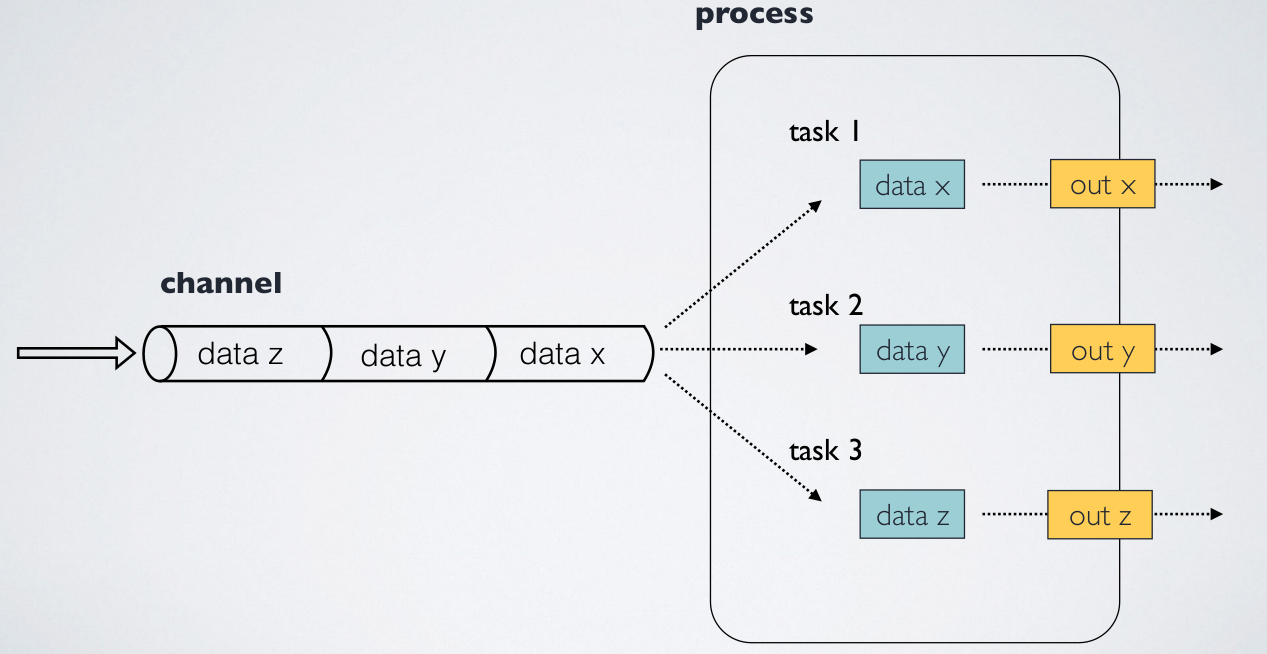
\includegraphics[width=.8\textwidth]{handout/channel-process.png}
\caption{Nextflow building blocks: a \emph{channel} ``feeding'' a processes. 
A \emph{task} is an instance of a process. An isolated task is created for each emission (data chunk) from the input channel. \emph{Credit: Evan Floden}}
\label{fig:proc-chn}
\end{figure}


\subsection{The script}

A nextflow script file name can be anything but in most cases it is best to stick to the default \texttt{main.nf}. 
The main script for the `hello' example is as follows:


\begin{lstlisting}
#!/usr/bin/env nextflow

cheers = Channel.from 'Bonjour', 'Ciao', 'Hello', 'Hola', 'Czesc'

params.universe = 'World'

process sayHello {
  echo true

  input:
    val cheer from cheers
    
  script:
    """
    echo "$cheer $params.universe!"
    """
}
\end{lstlisting}


A channel called \texttt{cheers} is created and emits each of the listed strings separately. 
A separate instance of the process \texttt{sayHello}, i.e.\ a \emph{task}, is executed for each emission. 

\begin{note}
The content of the above script can be broken down as follows:
\begin{itemize}
  \item The shebang line (line 1) is optional.
  \item \texttt{Channel.from(some\_list)} creates a channel emitting the list elements one by one.
  \item \texttt{params.universe = `World'} sets the default value of the command-line accessible option (e.g.\ \texttt{--world Mundo})
  \item \href{https://www.nextflow.io/docs/latest/process.html}{Process} definition (lines 7-16)
  \begin{itemize}
    \item Directives are placed at the top, directive \texttt{echo} controls whether \texttt{stdout} of the process is redirected to your terminal
    \item Input block (lines 10-11) 
    \item Script block (lines 13-16)
  \end{itemize}
  \item It is assumed to be a bash script unless an alternative shebang line (e.g.\  \texttt{/usr/bin/env python3}) is not specified at the top of the block 
  \item The \texttt{\$cheer} in the script block is a nextflow variable local to the process, \textbf{not} a bash variable.
  \item Indentation is inconsequential. 
\end{itemize}

\end{note}


\subsection{Hello HPC!}

The nextflow hello example shown us how the \texttt{sayHello} process was executed separately for each input string as a separate \emph{task}, but all the tasks were executed locally on our cluster's head node. 
We would now like each task to be submitted as a batch job for execution on one of the compute nodes.

Thanks to Nextflow's out-of-the-box support for different compute environments, 
it only requires changing the process executor from the default \texttt{local} to \texttt{slurm}.
This could be done via configuration files (more about that later) or using the directive \texttt{executor = `slurm'} in the process definition. 
However, for our simple use-case it should suffice to use the \texttt{NXF\_EXECUTOR} environmental variable.

\begin{steps}
\begin{lstlisting}
NXF_EXECUTOR=slurm nextflow run main.nf
\end{lstlisting}
\end{steps}

\begin{questions}
Play spot-the-difference -- how can you tell if the tasks were submitted on the cluster?
\begin{answer}
The terminal output should include the line \texttt{executor >  slurm (5)} (or similar), 
but may differ depending on the version of Nextflow and whether ANSI logging is switched on or off.
\end{answer}
\end{questions}

\begin{steps}
Let's modify our script slightly to make it easier to see how processes are executed.
Replace the single line within the script block

\begin{verbatim}
echo "$cheer $params.universe!"
\end{verbatim}

with the following

\begin{verbatim}
echo "$cheer ${params.universe}!  -- from ${task.executor} \$HOSTNAME"
\end{verbatim}
\end{steps}


\begin{warning}
Note the difference between how nextflow variables (\texttt{\$x,\$params.universe}) and bash variables (\texttt{\$HOSTNAME})are included in the script block.
There are alternative ways of including variables in scripts for execution by nextflow processes which may be more convenient if your script contains multiple special characters. See for example \href{https://www.nextflow.io/docs/latest/process.html#process-shell}{Nextflow documentation of the alternative \texttt{shell} block}\footnote{\url{https://www.nextflow.io/docs/latest/process.html\#process-shell}}. 
\end{warning}

\begin{steps}

Now re-run... 
\begin{lstlisting}
NXF_EXECUTOR=slurm nextflow run main.nf
\end{lstlisting}
\end{steps}

The messages printed to the terminal should now for each task include the executor being used and the name of the compute node on which the task was executed.







Nextflow facilitates but does not enforce separation of workflow logic from the configuration
of compute and software environments as well as from other properties of the workflow.  
As such, you \textit{could} get by developing nextflow workflows without worrying about that 
aspect -- but you would be missing a lot in terms of flexibility, extensibility, portability and more

Nextflow looks for workflow configuration primarily in \texttt{nextflow.config} file, and additional config files can be included. Unsurprisingly the `hello' example does not require much configuration,
we would also like to crunch some real, albeit small, data.

Let's have a play with a slightly more practical workflow.


\newpage


\section{Reimplementing a workflow in Nextflow}

In the Snakemake section of our tutorial, we include an example bash ``pipeline'', which 
includes a number of common tasks wrapped in a single 
\href{https://github.com/UofABioinformaticsHub/snakemake_template/blob/tutorial/analysis.sh}{bash script}\footnote{\url{https://github.com/UofABioinformaticsHub/snakemake_template/blob/tutorial/analysis.sh}}.
The workflow includes the following steps

\begin{itemize}
  \item Run FastQC across the raw read (FASTQ) files
  \item Adapter, quality, and read length filtering using Trimmomatic
  \item Aggregating FastQC reports from the raw reads using MultiQC
  \item Index the reference FASTA file
  \item Perform a \texttt{bwa-mem} read alignment
\end{itemize}

Before we start developing the Nextflow script, we need to set-up 
\begin{itemize}
  \item shared code base to to keep our efforts in sync
  \item input data for our workflow
  \item software environment including third-party tools
\end{itemize}



%------------------------
\subsection{Getting the code}
%------------------------

\begin{steps}
Start by cloning the workflow repository and moving to the directory.

\begin{lstlisting}
mkdir -p /shared/${USER}/nextflow
cd /shared/${USER}/nextflow
git clone https://github.com/csiro-crop-informatics/nextflow-embl-abr-webinar.git example_workflow
cd example_workflow
git checkout workshop
\end{lstlisting}
\end{steps}

%------------------------
\subsection{Getting the Data}
%------------------------

We have provided you with some real whole genome sequencing (WGS) data from bread wheat together with a small chunk of the wheat genome.
The data set is small enough for each step in the analysis to take less than a couple of minutes to run. 
We have a copy of this data available locally to save on bandwidth, time and the possibility we are detected as a DDoS attack on some poor remote server!

\begin{steps}
\begin{lstlisting}
# Get a copy of the data
cp --recursive \
  /shared/data/ \
  ./

# Have a look at what files we'd provided
tree data
\end{lstlisting}
\end{steps}

%------------------------
\subsection{The software environment}
%------------------------

There are multiple ways in which you can provision a software environment for your workflow.
You may have al the required tools installed on your system or available as a collection of pre-compiled binaries? Perhaps a friendly sysadmin installs convenient modules on your HPC cluster? You may also be using conda or perhaps docker or singularity containers? All those options are compatible with Nextflow. 
%The software environment for this workshop was put together using conda and captured in a Singularity container image. 

We have provided a rudimentary script \texttt{versions.nf} which tries to run each of the software tools,
and report their version numbers. 


\begin{steps}
Try to run
\begin{lstlisting}
nextflow run versions.nf
\end{lstlisting}
\end{steps}

\begin{warning}
This is expected to fail.\\
Unless all the software required by the pipeline is available on the \texttt{\$PATH},
which we don't expect, the pipeline should terminate with an error.
The output information may help you identify the cause. 
Try to relate the error message to the relevant section of the main script (\texttt{main.nf}). 
\end{warning}


\begin{questions}
Identify the exact \texttt{error}. 
\begin{answer}
The cause was likely ``\texttt{.command.sh: line 2: bwa: command not found}''. 
See line 23 in the following example:

\begin{lstlisting}
N E X T F L O W  ~  version 19.04.0
Launching `versions.nf` [elegant_morse] - revision: 525c4d8fea
[warm up] executor > local
[0a/26fff6] Submitted process > get_versions
ERROR ~ Error executing process > 'get_versions'

Caused by:
  Process `get_versions` terminated with an error exit status (127)

Command executed:

  fastqc --version
  multiqc --version
  echo -n "bwa " &&  bwa 2>&1 | grep 'Version'
  echo -n "samtools "&&  samtools 2>&1 | grep 'Version'

Command exit status:
  127

Command output:
  (empty)

Command error:
  .command.sh: line 2: fastqc: command not found

Work dir:
  /shared/training001/nextflow/example_workflow/work/0a/26fff6b11f473b0c3f0b3961608462

Tip: view the complete command output by changing to the process work dir and entering the command `cat .command.out`

 -- Check '.nextflow.log' file for details

\end{lstlisting}
\end{answer}
\end{questions}


There are different ways in which we could ensure that the relevant software is available, for example using process 
\emph{directives} at the top of each process definition. We could also use the opportunity to change the executor from local to Slurm, for example:
\begin{lstlisting}
process foo {
  module 'samtools/1.9' 
    executor 'slurm' 
  //further code omitted 
\end{lstlisting}

This is a perfectly valid syntax, which can be convenient, particularly during pipeline development, 
but for more portable workflows it is preferable to keep compute and software environment configuration 
separate from pipeline logic -- in simple terms not in the workflow script (\texttt{main.nf}).

\subsection{The config file(s) and profiles}

Workflow configuration belongs in \texttt{nextflow.config} file. 
Transferring the above mention \emph{directives} from process definitions in \texttt{main.nf} 
to \texttt{nextflow.config} would make things slightly better, e.g.

\begin{lstlisting}
#nextflow.config

process.executor = 'slurm' 
process.module = 'samtools/1.9' 
\end{lstlisting}

or using the preferred syntax

\begin{lstlisting}
process {
  executor = slurm
  module = 'samtools/1.9'
}
\end{lstlisting}


This is however still a bit rigid. 
\begin{itemize}
\item You may be developing your pipeline on a local machine or a server where software modules are not available. 
\item If developing directly in the cluster environment, you may prefer your quick test runs to happen either on the head node or in an interactive session you are using, rather than always having jobs submitted to sit in the always-busy cluster queue.
\end{itemize}

Nextflow enables the definition of \emph{profiles} which make it easy to run a workflow 
with different configuration settings, including, but not limited to executors and software environment.

For our pipeline we have defined several \emph{profiles}, which allow us to execute the logic from \texttt{main.nf} while providing the required software either by creating a \texttt{conda} environment or by using Docker of Singularity containers where the conda environment has already been captured. 

\subsubsection{Relevant profiles}


Have a look inside \texttt{nextflow.config}, and locate the process definitions

\begin{steps}
\begin{lstlisting}
less nextflow.config
\end{lstlisting}
\end{steps}

The ones most immediately relevant are:

\begin{lstlisting}
profiles {
  //EXECUTORS
  slurm {
    process {
      executor = 'slurm'
    }
  }
  //SOFTWARE
  conda {
    process {
      conda = "$baseDir/conf/conda.yaml"
    }
  }
  singularity {
    process {
      container = '/shared/.singularity/nextflow-embl-abr-webinar.simg' 
    }
    singularity {
      enabled = true
      autoMounts = true
    }
  }
}
\end{lstlisting}


As you can see, Nextflow makes it really easy to define software environment via Singularity 
or Conda\footnote{We also have a docker profile which you may find useful if you decide to run the workflow on your machine}. 


Given that Singlularity is available on our cluster, we will use the \texttt{singularity} profile for software environment using \texttt{-profile singularity}. Combinations of profiles can be selected at runtime 
so we will also use the \texttt{slurm} profile which will ensure the tasks are not executed on the head node but submitted to the cluster.

In addition to this basic configuration, there are many setting that can and in some cases must be set -- refer to 
\href{https://www.nextflow.io/docs/latest/executor.html}{executors section of Nextflow documentation}\footnote{\url{https://www.nextflow.io/docs/latest/executor.html}}. 
For running real-life pipelines in a cluster environment you will also use 
\href{https://www.nextflow.io/docs/latest/process.html#directives}{directives}\footnote{\url{https://www.nextflow.io/docs/latest/process.html\#directives}}
controlling the resources (\texttt{cpus, memory, time}) requested for each job. Other directives relevant in HPC context might include \texttt{queue} and \texttt{scratch}.



\begin{steps}
\begin{lstlisting}
# Load the Singularity module 
# If it is unavailable contact the cluster sysadmin

module load singularity-3.2.1-gcc-5.4.0-tn5ndnb

# Run the workflow

nextflow run versions.nf -profile slurm,singularity
\end{lstlisting}
\end{steps}


%\begin{questions}
%\begin{answer}
%\end{answer}
%\end{questions}

\section{Reimplementing a workflow in Nextflow - a walk-through}

Recall the steps of the original bash workflow

\begin{itemize}
  \item Run FastQC across the raw read (FASTQ) files
  \item Adapter, quality, and read length filtering using Trimmomatic
  \item Aggregating FastQC reports from the raw reads using MultiQC
  \item Index the reference FASTA file
  \item Perform a \texttt{bwa-mem} read alignment
\end{itemize}

We will walk you through reimplementing the first few steps 
into a Nextflow workflow. Along the way, we will introduce the core concepts of Nextflow 
and then ask you to reimplement the \texttt{bwa-mem} step yourselves. 
If you finish that with some time to spare, you will have the opportunity to reimplement the \texttt{multiqc} step. 
This will provide you with a foundation for you to be able to port your own workflows into Nextflow. 



%------------------------
\subsection{Implementing FastQC}
%------------------------

In this section you will learn how to 

\begin{itemize}
 \item Read multiple input files into a \emph{channel}
 \item View items emitted by a \emph{channel}
 \item Restrict how many items are emitted through a \emph{channel} using \emph{operators}
 \item Effortlessly parallelize the task by plugging a \emph{channel} into a \emph{process}
 \item Reference emitted items within processes' script block
\end{itemize}

\begin{steps}
Paste and save the following into a new file \texttt{main.nf}
\begin{lstlisting}
Channel.fromPath("data/raw_reads/*.fastq.gz")
  .view()
\end{lstlisting}

We create a (yet unnamed) channel and use the \texttt{view} \emph{operator} to
print the names of emitted files to the terminal. If you now run 


\begin{lstlisting}
nextflow run main.nf
\end{lstlisting}
\end{steps}

You will see a long list of files being emitted by the channel. 

While developing a workflow we tend to prefer to only use a small subset of data. 
We could restrict the number of FASTQ files emitted by the channel 
e.g.\ by pointing to a specific file or a subset of files, 
in this case the two read files available for Baxter

\begin{lstlisting}
Channel.fromPath("data/raw_reads/Baxter_R{1,2}.fastq.gz")
  .view()
\end{lstlisting}

We can do better! Let's use one of NF operators capable of limiting the number of items emitted by the channel.
Either \textbf{one} of \texttt{first()}, \texttt{last()} or \texttt{take(n)} will suffice.  


\begin{lstlisting}
Channel.fromPath("data/raw_reads/*.fastq.gz")
  .take(1) 
  .first() 
  .last() 
  .view()
\end{lstlisting}

Having all three operators is redundant, we will stick with \texttt{take(1)},
due to extra flexibility it gives us.
The last thing to do is to assign our channel to a variable whose name we can use elsewhere in the script.
The simplest form would be

\begin{lstlisting}
readsForQcChannel = Channel.fromPath("data/raw_reads/*.fastq.gz")
  .take(1)
  .view() 
\end{lstlisting}

But since we often chain multiple operations,
the following syntax is preferred due 
to consistent left-to-right flow.

\begin{lstlisting}
Channel.fromPath("data/raw_reads/*.fastq.gz")
  .take(1) 
  .view()
  .set { readsForQcChannel }
\end{lstlisting}


\begin{steps}
Update \texttt{main.nf} and run it again
\begin{lstlisting}
nextflow run main.nf
\end{lstlisting}
\end{steps}

You should see that only a single item is emitted by the channel.

Now that we have our input channel ready and emitting, we can remove the view operator
and focus on defining a process to implement the original bash snippet.

\begin{lstlisting}
fastqc \
  --threads 1 \
  raw_reads/${SAMPLE}_R1.fastq.gz \
  raw_reads/${SAMPLE}_R2.fastq.gz
\end{lstlisting}

In this case, there is no benefit from processing files as pairs.
In fact, separating the pairs should in principle allow more efficient 
allocation of resources as we will end up with twice the number of tasks,
but each being half the size of the original.


In \texttt{main.nf} we start our process definition by giving it a name 
and defining the input block 
\begin{lstlisting}
process fastqc {
    
  input:
   file(reads) from readsForQcChannel

}
\end{lstlisting}

We defined process input to be file taken from the \texttt{readsForQcChannel} which we assign to variable \texttt{reads}. We can now proceed to defining our script block.


\begin{lstlisting}
process fastqc {
    
  input:
   file(reads) from readsForQcChannel

  script:
  """
  fastqc --threads 1 ${reads}
  """
}
\end{lstlisting}

In the script block we address the input file via its variable name as \texttt{\$reads} or \texttt{\$\{reads\}}.

\begin{bonus}
Rather than fixing the number of threads inside the script block to 1, we could use the \texttt{task.cpus} variable. 

\begin{questions}
How can you set the value of the \texttt{task.cpus} variable? Hint: look into \emph{process directives} documentation.
\begin{answer}
\begin{lstlisting}
process fastqc {
  cpus 2
    
  input:
   file(reads) from readsForQcChannel

  script:
  """
  fastqc  --threads ${task.cpus} ${reads}
  """
}
\end{lstlisting}
\end{answer}
\end{questions}
\end{bonus}

%\begin{note}
%\begin{itemize}
% \item 
%
%% \item The (optional) \texttt{tag} directive will help us to decern   tag { reads.name }
%\end{itemize}
%\end{note}


%------------------------
\subsection{Implementing BWA Indexing}
%------------------------


In this section you will learn how to

\begin{itemize}
% \item  read an input file into a NF \emph{channel}
% \item  connect the created channel to NF \emph{process} input
% \item  port an existing bash snippet into NF \emph{process} script block
 \item  group \emph{process} output files and values in a \texttt{set} to be emitted through an output channel
\end{itemize}

In the original bash script this task consists of a simple call to \texttt{bwa} with 
the input fie name hard-coded. % also used for the prefix of the output filenames.

%bwa index -p references/reference.fasta.gz -a bwtsw references/reference.fasta.gz
\begin{lstlisting}
bwa index -a bwtsw references/reference.fasta.gz
\end{lstlisting}

We start by creating a channel which pass the reference file to our indexing process. 

\begin{lstlisting}
referencesChannel = Channel.fromPath('data/references/reference.fasta.gz') 

# or the equivalent

Channel.fromPath('data/references/reference.fasta.gz').set { referencesChannel } 
\end{lstlisting}

We can now move on to defining the process which will \emph{consume} the \texttt{referencesChannel}.

The bare-minimum would probably be a process definition with 
* an \texttt{input} block
* a \texttt{script} block

\begin{lstlisting}
process bwa_index {
  input:
    file(ref) from referencesChannel

  script:
  """
  bwa index -a bwtsw ${ref}
  """
}
\end{lstlisting}



%\begin{lstlisting}
%#!/usr/bin/env nextflow
%
%Channel.fromPath('data/references/reference.fasta.gz').set{ referencesChannel }
%
%process bwa_index {
%  input:
%    file(ref) from referencesChannel
%
%  output:
%    set val("${ref}"), file("*") into indexChannel 
%    
%  script:
%  """
%  bwa index -a bwtsw ${ref}
%  """
%}
%\end{lstlisting}

That should be sufficient to run the indexing, but given that we want to use the generated index,
in another process, we also need to define the outputs for the current one. 
The expected output files are:

\begin{lstlisting}
reference.fasta.gz.amb
reference.fasta.gz.ann
reference.fasta.gz.bwt
reference.fasta.gz.pac
reference.fasta.gz.sa
\end{lstlisting}

To capture these as outputs we could simply declare that all (non-input)
files constitute the desired output.

\begin{lstlisting}
  output:
    file("*") into indexChannel 
\end{lstlisting}

We could also be slightly more explicit and declare that outputs are all (non-input)
files sharing a prefix

\begin{lstlisting}
  output:
    file("${ref}.*") into indexChannel 
\end{lstlisting}

or even painstakingly list all the expected files... not recommended.
%and group them in a \emph{set} (in other words a tuple - an ordered list of elements).
%
%\begin{lstlisting}
%  output:
%    set file('reference.fasta.gz.amb'), file(reference.fasta.gz.ann), file('reference.fasta.gz.bwt'), file(reference.fasta.gz.pac), file(reference.fasta.gz.sa) into indexChannel 
%\end{lstlisting}
%
%
%However this is very verbose and 
However, one of the great things about Nextflow is that thanks to process isolation, 
you typically don't have to pay much attention to input/output file names 
unless a tool you use have some specific requirements in this regard.
For example, to run \texttt{bwa} alignment later on, we will need to pass it 
the common prefix of the names of the index files. 

In this case rather then simply outputting the index files,
and then parsing the prefix out of the file name(s), 
we opt to output our reference file name alongside the generated index file.
To do that in a single emission we wrap these in a \emph{set} 
(in other words a tuple - an ordered list of elements).

\begin{lstlisting}
  output:
    set val("${ref}"), file("*") into indexChannel 
\end{lstlisting}

The emitted set will consist of two elements 
\begin{itemize}
\item The reference file name (String) 
\item The list of index files (not just file names -- objects of class \texttt{java.nio.file.Path}).
\end{itemize}

This is our complete indexing process definition 
\begin{lstlisting}
process bwa_index {
  
  input:
    file(ref) from referencesChannel
  
  output:
    set val("${ref}"), file("*") into indexChannel 
    
  script:
  """
  bwa index -a bwtsw ${ref}
  """
}  
\end{lstlisting}

\begin{steps}
Give it a whirl,

\begin{lstlisting}
nextflow run main.nf -resume -profile slurm,singularity
\end{lstlisting}
\end{steps}

%------------------------
\subsection{Implementing Trimmomatic}
%---

We will guide you through the implementation of one more process before you take over!
The task is to adapter/quality trim raw reads as pairs and output them into a channel 
to be consumed by an alignment process.

The original bash implementation was as follows

\begin{lstlisting}
  #####
  mkdir -p qc_reads
  trimmomatic PE \
      -threads 1 \
      raw_reads/${SAMPLE}_R1.fastq.gz raw_reads/${SAMPLE}_R2.fastq.gz \
      qc_reads/${SAMPLE}_R1.fastq.gz qc_reads/${SAMPLE}_R1.unpaired.fastq.gz \
      qc_reads/${SAMPLE}_R2.fastq.gz qc_reads/${SAMPLE}_R2.unpaired.fastq.gz \
      ILLUMINACLIP:misc/trimmomatic_adapters/TruSeq3-PE.fa:2:30:10:3:true \
      LEADING:2 \
      TRAILING:2 \
      SLIDINGWINDOW:4:15 \
      MINLEN:36
\end{lstlisting}

This time we have to process the reads \textbf{as pairs} so using \texttt{Channel.fromPath()} 
will not suffice. Conveniently, NF has been developed by bioinformaticians so 
it smoothly handles paired files. 

\begin{lstlisting}
Channel.fromFilePairs("data/raw_reads/*_R{1,2}.fastq.gz")
  .take (1)
  .view ()
  .into { readPairsForTrimmingChannel }
\end{lstlisting}


\begin{note}
As before, during development we
\begin{itemize}
 \item use the \texttt{.take(n)} operator to limit the number of emissions coming through the channel
 \item use \texttt{.view()} to sneak-peak at what exactly is emitted
\end{itemize}
\end{note}

The output from the \texttt{.view()} operator in this case,
after some re-formatting would be something like

\begin{lstlisting}
[
  Gladius, 
  [
    /path/to/data/raw_reads/Gladius_R1.fastq.gz, 
    /path/to/data/raw_reads/Gladius_R2.fastq.gz
  ]
]
\end{lstlisting}

The single emission consists of a set of two elements. 
\begin{enumerate}
\item The sample name (accession) i.e. the file names prefix captured by the \texttt{`*'} glob. 
\item The list of two FASTQ files 
\end{enumerate}

One more thing we need, is a file containing the adapter sequences for trimmomatic.
This could be done in a number of ways, but it is best to stick to the dataflow paradigm 
and set-up another channel for that.

\begin{lstlisting}
Channel.fromPath('data/misc/trimmomatic_adapters/TruSeq3-PE.fa')
  .set{ adaptersChannel }
\end{lstlisting}

We now have two input channels, but how do we handle multiple input channels? 

If we just declare each separately 

\begin{lstlisting}
process trimmomatic {
  input:
    set val(accession), file(reads) from readPairsForTrimmingChannel
    file(adapters) from adaptersChannel
...    
\end{lstlisting}

This would work perfectly fine... but only for the first pair of reads. 
There is only a single adapters file emitted by the \texttt{adaptersChannel}, 
so once this channel no longer emits outputs, the process will not run again
and will never read the next pair of FASTQ files from \texttt{readPairsForTrimmingChannel}.

What we really want is for the adapters file to be used in combination with 
each pair of FASTQ files. Enter the \texttt{combine()} operator.

\begin{lstlisting}
process trimmomatic_pe {

  input:
    set file(adapters), val(accession), file(reads) 
      from adaptersChannel.combine(readPairsForTrimmingChannel)
...
\end{lstlisting}

This covers our inputs and we can now focus on the outputs and the script block.
As mentioned earlier we don't have to be too specific about the output file names 
but just have to make it clear to NF which output files are to be sent to an output channel.
In this case these are the ones with names ending with \texttt{paired.fastq.gz}.
We also output the \texttt{accession} variable to keep track of which sample is being processed.
%We do not have to use the \texttt{accession} and the output files could simply be named 
%\texttt{R1.paired.fastq.gz, ..., R2.unpaired.fastq.gz} or similar. 

\begin{lstlisting}
process trimmomatic_pe {

  input:
    set file(adapters), val(accession), file(reads) 
      from adaptersChannel.combine(readPairsForTrimmingChannel)
  output:
    set val(accession), file('*.paired.fastq.gz') into trimmedReadsChannel
...
\end{lstlisting}

The translation of the trimmomatic call from plain bash to bash embedded in the script block 
is straightforward. 

\begin{enumerate}
 \item Explicit paths to the input files are replaced with \texttt{\$\{reads\}} variable. The read files could also be addressed individually as \texttt{\$\{reads[0]\}} and \texttt{\$\{reads[1]\}}.
 \item Explicit output file paths for trimmomatic are replaced with convenient short names which need not be globally unique. 
\end{enumerate}



\begin{lstlisting}
process trimmomatic_pe {

  input:
    set file(adapters), val(accession), file(reads) 
      from adaptersChannel.combine(readPairsForTrimmingChannel)

  input:
    set file(adapters), val(accession), file(reads) from adaptersChannel.combine(readPairsForTrimmingChannel)

  output:
    set val(accession), file('*.paired.fastq.gz') into trimmedReadsChannel

  script:
  """
  trimmomatic PE \
    ${reads} \
    R1.paired.fastq.gz \
    R1.unpaired.fastq.gz \
    R2.paired.fastq.gz \
    R2.unpaired.fastq.gz \
    ILLUMINACLIP:${adapters}:2:30:10:3:true \
    LEADING:2 \
    TRAILING:2 \
    SLIDINGWINDOW:4:15 \
    MINLEN:36 \
    -Xms256m \
    -Xmx256m
  """
}
\end{lstlisting}


% \item The \texttt{\$\{reads\}} is the list comprised of the two input read files. These could be accessed individually using \texttt{\$\{reads[0]\}} and \texttt{\$\{reads[1]\}}.


%------------------------
\subsection{Implementing BWA-MEM}
%-

Now is your opportunity to put into practice what you have learnt from the above walk-
through of implementing FastQC and Trimmomatic commands. Your task is to implement
the \texttt{bwa mem} command in a Nextflow process.


The relevant snippet from the bash pipeline is as follows 
\begin{lstlisting}
  bwa mem -t 1 \
    references/reference.fasta.gz \
    qc_reads/${SAMPLE}_R1.fastq.gz qc_reads/${SAMPLE}_R2.fastq.gz \
  | samtools view -b \
  > mapped/${SAMPLE}.bam
\end{lstlisting}

Here are some questions to get you thinking 

\begin{questions}
The mapping process requires and index comprised of several files but takes their common prefix (basename) 
as argument. How can you pass that prefix to the command?\\
\begin{answer}
You \emph{could} hard-code it (not a good practice) or parse it out from the index file names. 
\end{answer}
Can you do it without hard-coding it or having to parse it out from the input file name(s)?\\
\begin{answer}
Our indexing process, in addition to the index files also outputs the prefix used when building the index. \\
\end{answer}
How do you make sure that each instance of the process - and not just the first one - gets the index files in \emph{(cough)} combination with a pair of FASTQ files?\\
\begin{answer}
Use the \emph{combine} operator to combine the \texttt{indexChannel} with the \texttt{trimmedReadsChannel}.
\begin{lstlisting}
process bwa_mem {
  input:
    
  output:
    
  script:
  """
  bwa mem -t ${task.cpus} ${ref} ${reads} \
  | samtools view -b > ${accession}.bam
  """
}
\end{lstlisting}
\end{answer}
\begin{answer}
\end{answer}
\end{questions}


%------------------------
\subsection{Adding New Samples}
%------------------------

Since we had to stop the channel from sucking up all the samples by applying the take operator 
we expect you may already know how to make sure all samples are processed.




%
%We are going to work with an example Nextflow workflow to demonstrate how they are run, 
%improve your understanding of \emph{processes} and \emph{channels} and finally introduce\ \emph{operators}, which are applied to channels to shape and direct flowing data.




\subsection{Under the hood}

If you think you are ready to look under the hood and try to work out how nextflow stages process inputs, wraps process script blocks and submits them to the cluster, here is a start. 

\begin{advanced}
\begin{lstlisting}
# Remove the work directory to limit the number of task directories to look at
rm -r work
# Re-run for a single sample
nextflow run main.nf -profile slurm,singularity
# Take a peak
ls -la work/ | less
# or
tree -ah work/ | less
\end{lstlisting}

Each task is executed in a separate directory and every abbreviated hash displayed in the terminal can be related to a specific sub-directory of \texttt{./work},\\ such as
\texttt{work/d2/c4517b0a81f61ceca29ec355ddeaa6/} in which you may find

\begin{lstlisting}
# NF generated files
.command.begin
.command.err
.command.log
.command.out
.command.run
.command.sh
.command.trace
.exitcode

# Output file
H45.bam

# Symlinks to input files
H45_R1.paired.fastq.gz
H45_R2.paired.fastq.gz
reference.fasta.gz.amb
reference.fasta.gz.ann
reference.fasta.gz.bwt
reference.fasta.gz.pac
reference.fasta.gz.sa
\end{lstlisting}

Identify and investigate hidden file (starting with dot) containing the executed script and the one containing cluster and container handling. 

%\begin{questions}
%
%\begin{answer}
%
%\end{answer}
%\end{questions}

\end{advanced}




\begin{bonus}
For an optional exercise you may try to re-run the workflow with \texttt{conda}.
For that, you'll need to find and load a conda module before re-running the workflow with appropriate profile. Don't forget to use the \texttt{-resume} flag.
\begin{answer}
\begin{lstlisting}
# Find the appropriate module name
module av -l 2>&1 | grep conda

# Load the module
module load miniconda3-4.6.14-gcc-5.4.0-kkzv7zk

# Run with conda
nextflow run main.nf -profile conda,slurm --take all -resume

\end{lstlisting}
\end{answer}

If you remembered to use \texttt{-resume}, why do you think it appeared to not make a difference?

\begin{answer}
We have switched from singularity to conda so the software environment has changed.  
\end{answer}


\end{bonus}




%\begin{figure}[H]
%\centering
%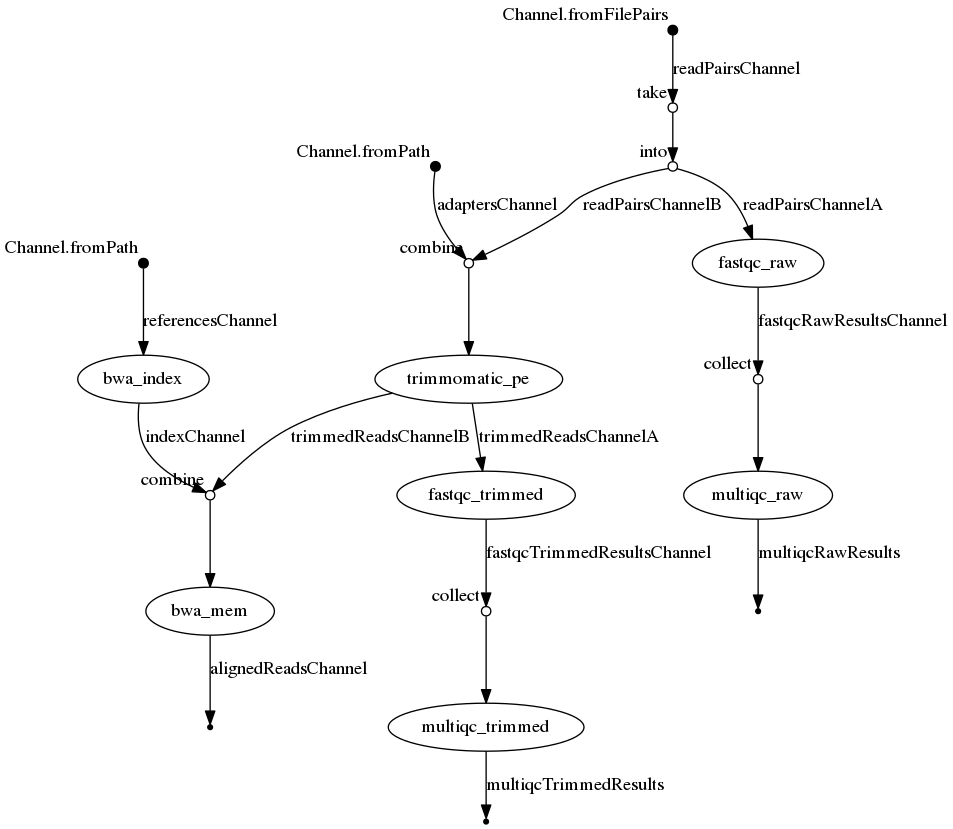
\includegraphics[width=\textwidth]{handout/flowchart.png}
%\caption{The example workflow}
%\label{fig:dag}
%\end{figure}
%
%
%\begin{questions}
%Investigate \texttt{main.nf} alongside Figure~\ref{fig:dag}. 
%
%Which \href{https://www.nextflow.io/docs/latest/operator.html}{nextflow operators}\footnote{\url{https://www.nextflow.io/docs/latest/operator.html}}, in addition to the previously discussed, are used and for what purposes? 
%
%\begin{answer}
%The \texttt{.combine()} operator outputs all combinations of items emitted by two channels. This results with a downstream process to be executed for each such combination. So e.g. \texttt{bwa\_mem} will be executed for\\ $(reference, accession_1),(reference, accession_2),..,(reference, accession_n)$.
%
%The \texttt{.collect()} operator collects all the items emitted by a channel returns the resulting \texttt{List} as a single emission. This is required e.g.\ if a process needs to be executed once with all the samples as input.
%\end{answer}
%
%\end{questions}


\subsection{Workflow outputs}

We now now each task is nicely isolated in a separate sub-directory under \texttt{work}, but how do I find my results? Was it \texttt{work/a7:fc9339a827fb4b34d2408e1c3ee29c} or maybe \texttt{work/3c:8fdf958e96b448ecb83bd7806af382}? This should be handled by applying the \href{https://www.nextflow.io/docs/latest/process.html#publishdir}{\texttt{publishDir} directive}\footnote{\url{https://www.nextflow.io/docs/latest/process.html\#publishdir}} to selected processes. As with other directives, this can be included at the top of the process block or in a configuration file using \href{https://www.nextflow.io/docs/latest/config.html#process-selectors}{process selectors}\footnote{\url{https://www.nextflow.io/docs/latest/config.html\#process-selectors}} to apply the directive to one or more relevant process. To keep things tidy-ish, we define the publishing of the outputs in a separate file 
which we \texttt{includeConfig 'conf/publish.config'} in \texttt{nextflow.config}. 

In \texttt{conf/publish.config} we only really use the \texttt{withName} selectors.
The alternative \texttt{withLabel} selectors are convenient e.g.\ when outputs of multiple 
processes are to be gather in one location, in which case we attach the same \texttt{label} to each of those processes.

%\begin{bonus}
%In \texttt{conf/publish.config} we only really use the \texttt{withName} selectors. 
%
%\end{bonus}

\subsection{Cluster run - all accessions}

We have successfully submitted workflow to the cluster. 

To be sure, feel free to re-run it again (and again, and again...) 
with \texttt{-resume} to avoid wasting CPU cycles.

\begin{steps}
\begin{lstlisting}
nextflow run main.nf -profile slurm,singularity -resume
\end{lstlisting}
\end{steps}

If all went well, the workflow successfully processed a single accession, 
let's have a closer look at the script to better understand how it handles 
the inputs before we proceed to run it on all the accessions.

\begin{questions}
In \texttt{main.nf} we create a channel which reads pairs of FASTQ files from a sub-directory of the \texttt{./data}. We then apply some operators. 
\begin{verbatim}
Channel.fromFilePairs("data/${region}/*_R{1,2}.fastq.gz")
  .take ( params.take == "all" ? -1 : params.take ) 
  .into { readPairsChannelA; readPairsChannelB } 
\end{verbatim}
1. Identify the two operators, refer to 
\href{https://www.nextflow.io/docs/latest/operator.html}{nextflow documentation}\footnote{\url{https://www.nextflow.io/docs/latest/operator.html}}
as required and explain the purpose of each of the two operators.\\
\begin{answer}
\texttt{.take($n$)} limits the number of emissions from the channel to the first $n$ items. \\
\texttt{.into\{ $ch_1;ch_2;...;ch_n$ \}} creates channels $ch_1,ch_2,...,ch_n$ and connects source channel to the newly created channels, so that every emission is sent through each new channel.
\end{answer}

2. How can you run the workflow for more than one accession? How about all of them? Recall that workflow parameters use double-dash syntax. Run the relevant commands.  
\begin{answer}
\begin{lstlisting}
nextflow run main.nf -profile slurm,singularity -resume --take 2
nextflow run main.nf -profile slurm,singularity -resume --take all
\end{lstlisting}
\end{answer}
%3. Investigate \texttt{main.nf} to identify the processes which consume \texttt{readPairsChannelA} and \texttt{readPairsChannelB}. \\
%
%Q????
%
\end{questions}

\subsubsection{Monitoring your jobs on our cluster}

\begin{note}
You can monitor your job(s) in the slurm queue using the slurm command \texttt{squeue}:

\begin{lstlisting}
squeue --user ${USER}
\end{lstlisting}

For convenience you are also provided with the \texttt{sq} function which produces nicer output and by default only shows your own jobs:

\begin{lstlisting}
sq

# Someone elses jobs
sq --user ${SOMEONE_ELSE}
\end{lstlisting}

If you want to see all jobs in the queue:

\begin{lstlisting}
squeue
\end{lstlisting}

\end{note}


\section{Modify/extend the workflow}

\begin{steps}

Edit \texttt{main.nf}. Your task is to add a process which will merge the bam files produced by the \texttt{bwa\_mem} process. 

\begin{questions}
How do you ensure that \textbf{all} BAM files end up in the same instance of your process?
\begin{answer}
Using the \texttt{.collect()} operator.
\end{answer}
Demonstrate your process definition to your facilitator.

\begin{answer}
\begin{lstlisting}
process bam_merge {
  input:
    file('*.bam') from alignedReadsChannel.collect()

  script:
  """
  samtools merge ${params.take}_accessions_megred.bam *.bam
  """
}
\end{lstlisting}
\end{answer}
Where can we find the merged BAM file? Can you publish it to a human-readable location? Hint: only declared outputs can be published.
\end{questions}

\begin{bonus}
\begin{questions}
Modify your merge process to allow samtools to use 2 cpus with \texttt{--threads 2},
don't forget to modify your process configuration to request 2 cpus per task.
\end{questions}
\end{bonus}


\end{steps}



%% To make a paragraph appear as a "note" to the reader, simply wrap it in a "note" environment like
%% this:
%\begin{note}
%Note that currently the default behaviour of Nextflow is to re-run an entire workflow 
%unless \texttt{-resume} option is specified at run-time, in which case a previously 
%executed process is not re-run if all its inputs remain unchanged.
%
%\end{note}



%========================
\section{Troubleshooting}
%========================

\subsection{Disconnected from the cluster?}  

\subsection{Missing modules - new shell session?}



Make sure all the required modules are loaded. 

\begin{steps}
\begin{lstlisting}
# Java - essential for nextflow
module load openjdk-1.8.0_202-b08-gcc-5.4.0-sypwasp 

# Singularity - our go to system for providing software for the example workflow
module load singularity-3.2.1-gcc-5.4.0-tn5ndnb


# If using conda 
module load miniconda3-4.6.14-gcc-5.4.0-kkzv7zk
\end{lstlisting}
\end{steps}




